% !TeX program = pdflatex
% !BIB program = bibtex
\documentclass[10pt,conference,letterpaper]{IEEEtran}

\usepackage[T1]{fontenc}
\usepackage[utf8]{inputenc}
\usepackage{amsmath,amssymb}
\usepackage{booktabs}
\usepackage{cite}
\usepackage{graphicx}
\usepackage{siunitx}
\usepackage{tabularx}
\usepackage{tikz}
\usetikzlibrary{arrows.meta,positioning}
\usepackage{xurl}
\usepackage[hidelinks]{hyperref}
\urlstyle{same}
\sisetup{detect-all=true}
\hypersetup{
  pdftitle={Channel Knowledge Maps for FR3 UAV Base Stations: Dataset and ML-Based Modeling},
  pdfauthor={Guillem Moreno Garcia, Sergi Abadal, Evgenii Vinogradov}
}

\title{Channel Knowledge Maps for FR3 UAV Base Stations: Dataset and ML-Based Modeling}

\author{\IEEEauthorblockN{Guillem Moreno Garcia, Sergi Abadal, Evgenii Vinogradov}
\IEEEauthorblockA{Universitat Polit\`ecnica de Catalunya (UPC), Barcelona, Spain\\
guillem.moreno.garcia@estudiantat.upc.edu}}

\begin{document}
\maketitle

\begin{abstract}
This paper introduces a dense FR3 channel knowledge map (CKM) dataset for
unmanned aerial vehicle base stations. It contains 16180 ray-traced
layout--height combinations from 3236 urban locations in 66 cities at
\SI{7.125}{GHz}. Every $513\times513$ realization stores building geometry,
geometric visibility, attenuation, delay spread, angular spread, and a
variable transmitter height. As a focused first benchmark, we propose an
interpretable height-aware attenuation model. Its line-of-sight branch combines
free-space loss with a coherent image-source two-ray term and compact
height/range calibration. Its non-line-of-sight branch combines a
COST231-shaped basis with local morphology and topology-specific linear
calibration. Under a strict city holdout, the frozen model reaches
\SI{1.9289}{dB} overall root mean square error, with \SI{1.7370}{dB} in LOS and
\SI{3.5363}{dB} in NLOS, on 2590 maps from 14 unseen cities. Its median CPU
time is \SI{0.0602}{s} per map. The result provides a transparent attenuation
baseline and a physical anchor for later distribution-aware refinement of all
three channel quantities.
\end{abstract}

\begin{IEEEkeywords}
channel attenuation, channel knowledge map, delay spread, path loss, radio map,
unmanned aerial vehicle.
\end{IEEEkeywords}

\section{Introduction}
Uncrewed aerial vehicles (UAVs) carrying base stations can support future 6G
networks through mobility and an increased probability of line of sight (LOS).
Their deployment nevertheless requires
fast, location-dependent channel information for placement and resource
management. Channel knowledge maps (CKMs) address this need by indexing
channel information by transmitter or receiver location
\cite{ckmtutorial2024,zengx2021ckm}.

Dense CKMs can be measured or simulated. Measurements are costly to collect at
scale, whereas deterministic ray tracing (RT) provides spatially complete
labels at substantial computational cost. Learned surrogates such as
RadioUNet and PMNet therefore use convolutional encoder--decoders to predict
dense maps from city geometry and transmitter information
\cite{radiounet2020,pmnet2023}. Existing datasets, however,
predominantly use fixed terrestrial transmitters and omit spatially varying
building height.

The upper mid-band frequency range, FR3, is being studied as a
coverage/capacity bridge for 6G~\cite{Cui2024}. It is attractive for UxNB
deployment, but blocked links remain relevant even with elevated transmitters.
Assessing this setting requires height-aware channel data across diverse urban
environments. To our knowledge, no public CKM dataset currently combines FR3,
UxNB-specific geometry, and dense three-dimensional building information.

\begin{table*}[t]
\centering
\caption{Comparison of dense CKM and radio-map datasets.}
\scriptsize
\setlength{\tabcolsep}{4pt}
\begin{tabular}{@{}lcccc@{}}
\toprule
Property & This work & UrbanRadio3D~\cite{radiodiff3d2026} & RadioMapSeer~\cite{dataset2212} & CKMImageNet~\cite{ckmimagenet2025} \\
\midrule
Variable elevated Tx height & yes & no & no & no \\
Layout groups or maps & 3236 groups & 701 & 701 & 40000 \\
Raster size(s) & $513^2$ & $256^2$ & $256^2$ & $32^2$--$128^2$ \\
Horizontal resolution & 1 m & 1 m & 1 m & 2 m \\
Channel quantities & Att. (PL), LOS, DS, AS & PL, DoA, ToA & PL & Gain, AoA/AoD, delay \\
Building-height raster included & yes & yes & no & no \\
Per-sample topology labels & 3 and 6 classes & no & no & no \\
\bottomrule
\end{tabular}
\label{tab:datasets}
\vspace{-8pt}
\end{table*}

\paragraph{Limitations of the existing CKM datasets}
Table~\ref{tab:datasets} compares the learning inputs distributed by each
dataset rather than the provenance of its source geometry. Here, 3236 location
groups paired with five transmitter heights produce 16180 realizations.
``Building-height raster'' means that every building pixel retains a height,
rather than only a binary footprint; it does not imply that every height was
surveyed directly. We combine global products providing both footprint and
height~\cite{Che2024globfp,Zhu2025atlas}, avoiding the sparse height tags in
OpenStreetMap~\cite{Bernard2022}.

\begin{figure*}
\centering
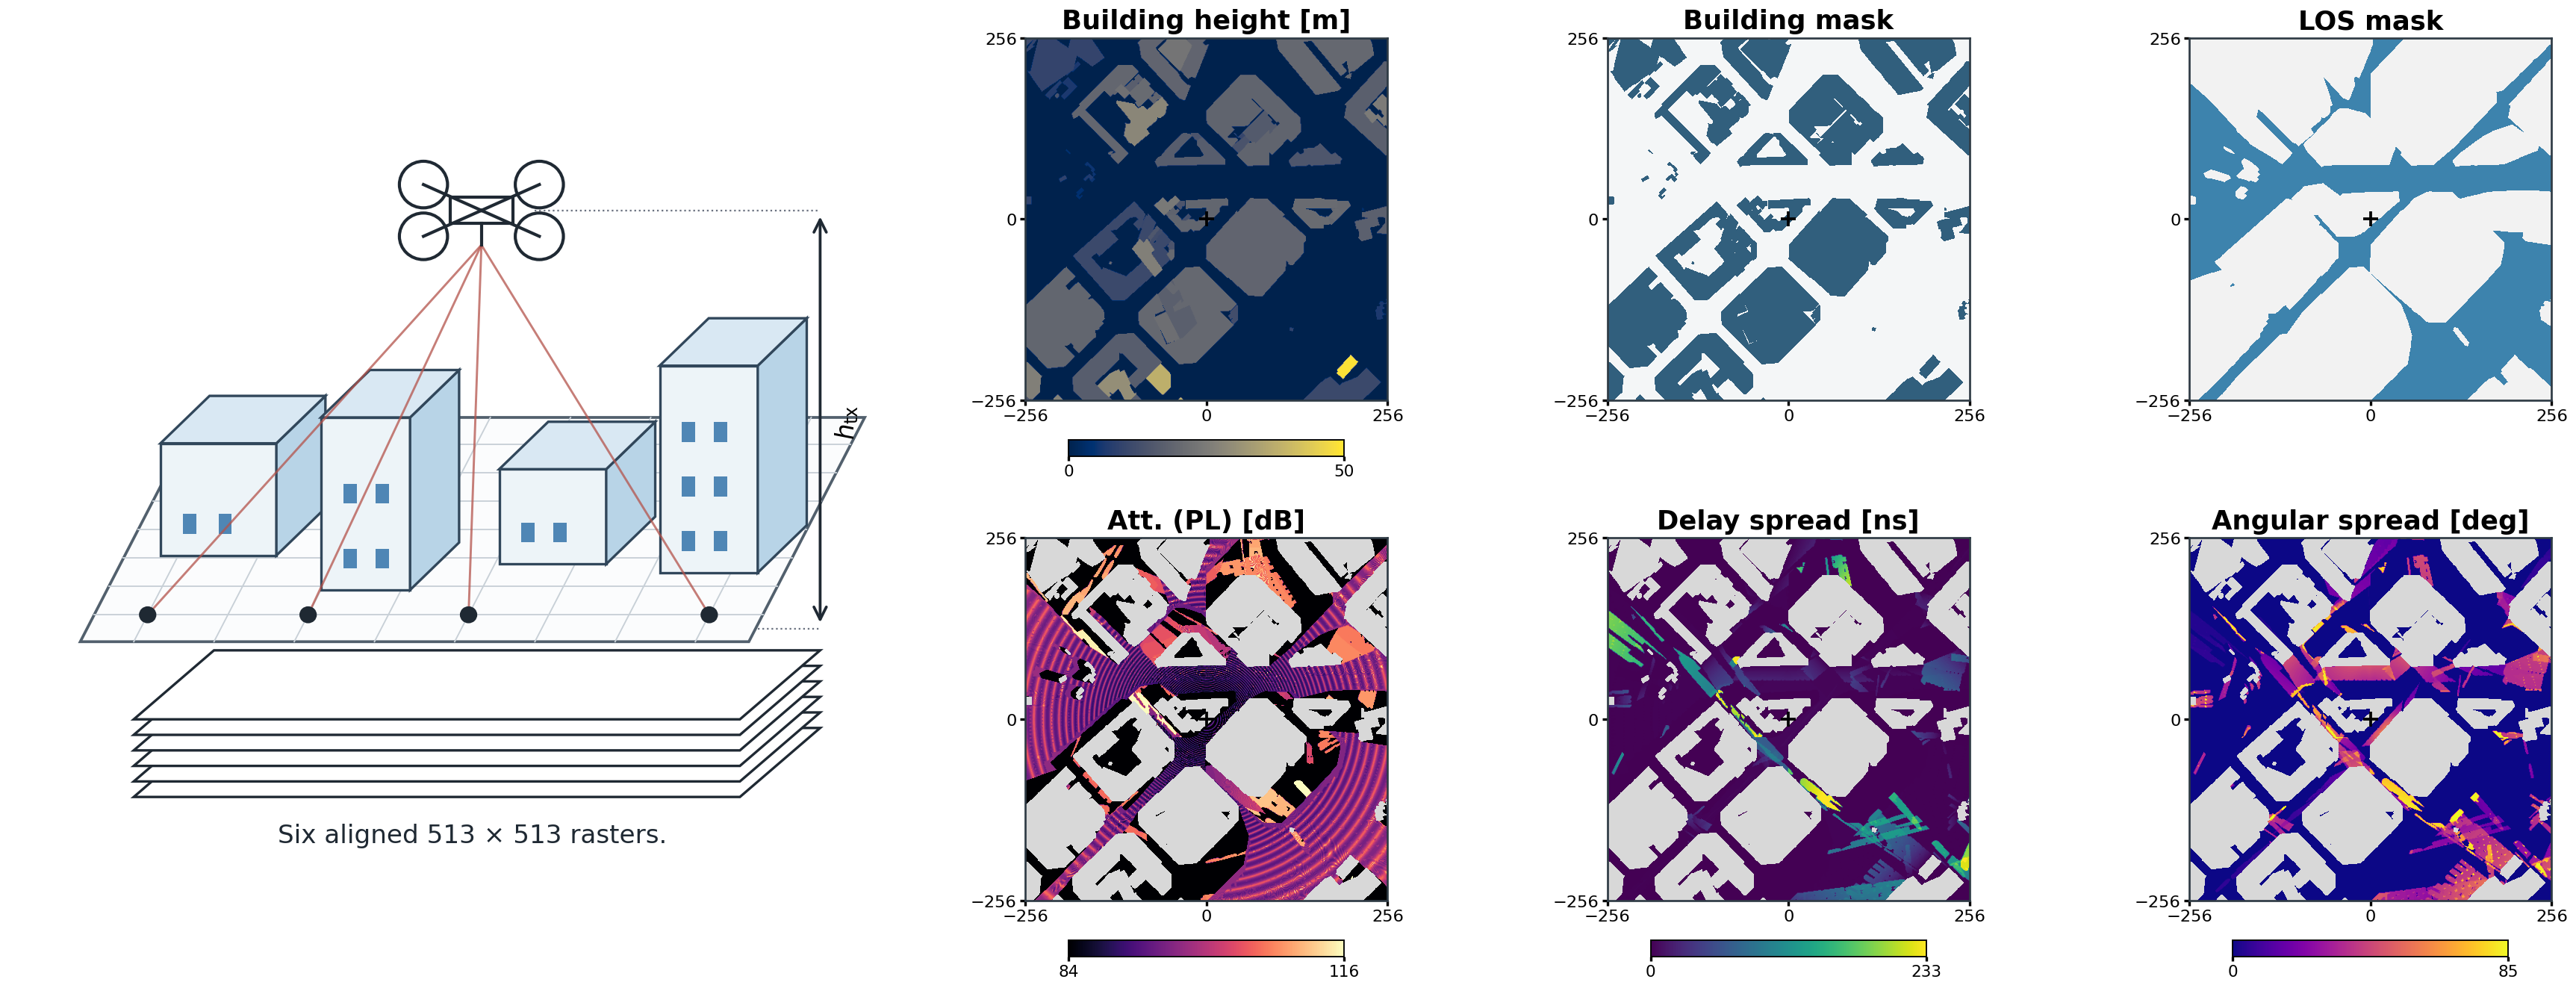
\includegraphics[width=\textwidth]{figures/ckm_dataset_real_sample.png}
\caption{One Barcelona realization (\texttt{sample\_02806}) at
$h_{\mathrm{tx}}=\SI{69.4}{m}$. The left illustration shows an elevated UxNB
above six aligned $513\times513$ rasters. The panels show building height,
building mask, LOS, attenuation, delay spread, and angular spread. Crosses mark
the centered transmitter; gray areas are building pixels excluded from the
metrics. For this sample, the stored three- and six-class labels are
\texttt{dense\_highrise} and \texttt{dense\_block\_midrise}.}
\label{fig:ckm_sample}
\vspace{-8pt}
\end{figure*}

A UxNB CKM should cover a typical cell diameter of 300--500 m with a spatial
resolution capable of capturing relevant variations over approximately
20--80 wavelengths~\cite{saboor26}. Since UxNB heights can approach 500 m,
their channels differ substantially from fixed terrestrial links. UrbanRadio3D includes receiver heights
up to 20 m~\cite{radiodiff3d2026}, but does not provide the continuously varying
elevated-transmitter geometry considered here. Accurate building height is
particularly important because it controls visibility and rooftop blockage.

\paragraph{Limitations of the existing CKM modeling approaches}
Dense attenuation is commonly treated as unconstrained image-to-image
regression. This asks large networks to relearn stable propagation structure,
often under fixed terrestrial geometry, and obscures whether they transfer to
unseen cities and continuously varying UxNB heights.

\paragraph{Beyond state-of-the-art contributions}
In this paper, we address these gaps. The main contribution thus is two-fold:
\begin{enumerate}
    \item We introduce a \SI{7.125}{GHz} Channel Knowledge Map dataset generated via ray-tracing simulations in 3,236 city layouts across 66 diverse cities. This dataset relies on global-scale 3D building data~\cite{Che2024globfp,Zhu2025atlas}. UxNB applications are enabled by using five transmitter heights per layout, resulting in 16180 CKM samples.
    \item We propose a height-aware channel prediction framework\footnote{The
    dataset contains attenuation, angular spread, and delay spread; this first
    benchmark predicts attenuation only.} that separates LOS and NLOS
    propagation using local city geometry. Free-space, coherent two-ray, and
    COST231/Hata-derived terms are calibrated through compact lookup tables and
    ridge regression, enabling zero-shot transfer to unseen cities.
\end{enumerate}

\textbf{Notation:} Bold uppercase symbols denote rasters or tensors, bold
lowercase symbols denote vectors, and $\odot$ is element-wise multiplication.

\section{CKM: Definition and Dataset Description}
\label{sec:ckm_dataset}

Figure~\ref{fig:ckm_sample} illustrates one sample from the dataset. In the
following, UxNB and transmitter are used interchangeably.

\subsection{CKM Definition and Mapping Formulation}
\label{sec:ckm_def}
For realization $n$, let $\mathbf E_n\in\mathbb R^{H\times W\times L}$
contain environmental layers, $\mathbf C_n\in\mathbb R^{H\times W\times F}$
contain channel quantities, and $\mathbf m_n\in\mathbb R^K$ contain metadata.
CKM estimation seeks a mapping
\begin{equation}
\widehat{\mathbf C}_n=\mathbf\Phi_{\boldsymbol\theta}
(\mathbf E_n,\mathbf m_n),
\label{eq:mapping_generic}
\end{equation}
where $H=W=513$, $L=2$, and $F=4$.

\subsection{The FR3 UxNB CKM Dataset}
\label{sec:dataset_details}
We construct a comprehensive benchmark dataset using high precision deterministic simulations.

\subsubsection{3D Urban Environment Modeling}
\label{sec:env_model}
The environmental tensor $\mathbf E_n$ combines GlobalBuildingAtlas and
3D-GloBFP~\cite{Che2024globfp,Zhu2025atlas}. Unlike optional OpenStreetMap
height tags, whose availability is below 10\%~\cite{Bernard2022}, these products
provide both building footprint and height. This information is necessary to
represent how UxNB altitude changes rooftop blockage and visibility.

We extract city layouts of 3,236 urban locations in 66 diverse cities worldwide to cover a range of propagation topologies (from open low-rise suburbs to dense high-rise downtown areas). Each rasterized environmental map $\mathbf{E}_n$ spans a spatial grid of $H = W = 513$ at a horizontal resolution of $1\text{~m}$. The $L=2$ environmental channels encode:
\begin{enumerate}
    \item Building height profile maps $\mathbf{H}$ indicating building height in meters ($0\text{~m}$ over ground level).
    \item Binary building occupancy masks $\mathbf{B}$ indicating presence of structural obstacles.
\end{enumerate}

\subsubsection{Ray Tracing Channel Simulation}
\label{sec:rt_sim}
High precision ray tracing simulations are conducted to generate the spatially consistent channel tensors $\mathbf{C}_n$. To avoid using separate software for 3D model construction (e.g., Blender) and for RT (e.g., Wireless InSite or Sionna), SiteViewer and RT capabilities of MATLAB are used in this work. %Note that MATLAB RT is slightly slower than the mentioned commercial and open solutions~\cite{Zhu2024RT}.

RT simulation parameters are summarized in Table~\ref{tab:rt_params}. The
\SI{7.125}{GHz} frequency is a WRC-23 candidate band available across all ITU
regions, while the \SI{1}{m} resolution corresponds to approximately 24
wavelengths~\cite{saboor26}. The UxNB is horizontally centered and evaluated at
five independently sampled heights per location. The observed range is
approximately \SIrange{12}{478}{m}, yielding $N=16180$ samples. Receivers are
placed at \SI{1.5}{m} over every non-building coordinate. The channel tensor
stores $F=4$ channels:
\begin{enumerate}
    \item Binary visibility mask $\mathbf{V}$: LOS ($1$) vs. NLOS ($0$) states.
    \item Channel attenuation in dB.
    \item Multi-path RMS delay spread in ns.
    \item  Multi-path RMS angular spread in degrees.
\end{enumerate}
Building elements are assigned zero in $\mathbf{C}_n$ and are excluded from
training and evaluation.

\subsubsection{Metadata}
\label{sec:metadata}

Because carrier frequency, receiver height, and horizontal transmitter location (fixed at the grid center) are constant across all simulations, the metadata vector $\mathbf{m}_n$ consists of:
\begin{enumerate}
    \item Transmitter height $h_{\text{tx}}$, observed from approximately \SIrange{12}{478}{m}.
    \item Categorical tags mapping the layout to three- and six-class
    morphology partitions. The attenuation model recomputes its three-class
    ITU route from the raster as described in Section~\ref{sec:nlos}.
\end{enumerate}

The three deployed ITU topology prototypes and the resulting support in the
complete dataset are:
\begin{center}
\small
\begin{tabular}{|l|c|c|c|c|}
\hline
Topology & Samples & $\alpha$ & $\beta$ [km$^{-2}$] & $\gamma$ [m] \\ \hline
Suburban & 7,435 & 0.1 & 750 & 8 \\ \hline
Urban & 7,350 & 0.3 & 500 & 15 \\ \hline
Dense Urban & 1,395 & 0.5 & 300 & 20 \\ \hline
\end{tabular}
\end{center}
Here, ``Samples'' counts all 16,180 realizations. Each of the 3,236 layouts
contributes its five transmitter heights to the same topology class.

\begin{table}[t]
\centering
\caption{Ray-tracing simulation parameters.}
\label{tab:rt_params}
\begin{tabular}{ll}
\hline
{Parameter} & {Value} \\ \hline
Carrier frequency, $f$ & \SI{7.125}{GHz} \\
Antenna model & Isotropic \\
Sample dimensions & $513\times513$ at \SI{1}{m} \\
Ground receiver height, $h_{\text{rx}}$ & \SI{1.5}{m} \\
Observed transmitter height, $h_{\text{tx}}$ & \SIrange{12}{478}{m} \\
UxNB heights per location & 5 \\
Total CKM samples, $N$ & 16,180 \\
\hline
\end{tabular}
\end{table}

The labeled HDF5 file stores both three- and six-class topology tags and the
transmitter-height bin alongside the six rasters. Generation and model code are
publicly available.\footnote{\url{https://github.com/unworthyzeus/CKMGenerator};
\url{https://github.com/unworthyzeus/Final_Code_TFG}.}
% TODO(camera ready): add the persistent IEEE DataPort or Zenodo dataset DOI.

\section{Height-Aware CKM Modeling}\label{sec:ckm_model}

\begin{figure}[t]
\centering
\resizebox{\columnwidth}{!}{%
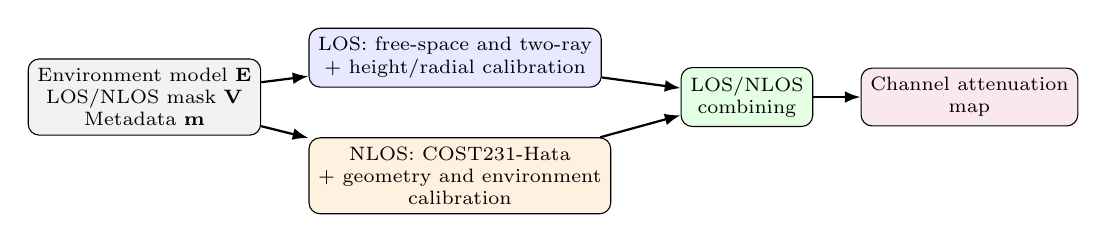
\begin{tikzpicture}[
node distance=5mm and 6mm,
box/.style={draw,rounded corners,align=center,minimum height=7mm,font=\scriptsize},
arr/.style={-{Latex[length=2mm]},thick}]
\node[box,fill=gray!10] (input) {Environment model $\mathbf E$\\LOS/NLOS mask $\mathbf V$\\Metadata $\mathbf m$};
\node[box,fill=blue!9,right=of input,yshift=5mm] (los) {LOS: free-space and two-ray\\+ height/radial calibration};
\node[box,fill=orange!12,right=of input,yshift=-10mm] (nlos) {NLOS: COST231-Hata\\+ geometry and environment\\calibration};
\node[box,fill=green!10,right=10mm of los,yshift=-5mm] (switch) {LOS/NLOS\\combining};
\node[box,fill=purple!9,right=of switch] (out) {Channel attenuation\\map};
\draw[arr] (input) -- (los);
\draw[arr] (input) -- (nlos);
\draw[arr] (los) -- (switch);
\draw[arr] (nlos) -- (switch);
\draw[arr] (switch) -- (out);
\end{tikzpicture}}
\caption{The proposed solution uses separate LOS and NLOS propagation models calibrated with training CKM data.}
\label{fig:CKM_model}
\end{figure}

In this section, we propose a propagation physics-informed CKM attenuation
simulator (see Fig.~\ref{fig:CKM_model}). The model implements the
attenuation-focused mapping function $\mathbf\Phi_{\boldsymbol\theta}
(\mathbf E_n,\mathbf m_n)$ by modeling LOS and NLOS attenuation separately:
\begin{equation}
\boldsymbol\Lambda=\mathbf V\odot\boldsymbol\Lambda_{\mathrm{LOS}}
 +(1-\mathbf V)\odot\boldsymbol\Lambda_{\mathrm{NLOS}},
\label{eq:combined}
\end{equation}
where $\odot$ denotes element-wise multiplication for masking. The LOS model
uses free-space and coherent two-ray propagation corrected with terms learned
from the CKM dataset. The NLOS model uses the ITU topology characteristics and
a CKM-calibrated COST231-Hata basis. The visibility mask $\mathbf V$ is the
binary output of the configured MATLAB ray tracer, not a prediction of the
attenuation model; for matching geometry and RT settings, it can be stored once
and reused. All calibration tables and regression weights are fitted using
training cities and frozen before evaluating a held-out city.

Given the deployment geometry ($h_{\text{tx}}$, $h_{\text{rx}}$, and the fixed horizontal UxNB position), we pre-compute spatial geometry matrices over the $513 \times 513$ grid: horizontal distance $\mathbf{D}_{\text{2D}}$, direct 3D distance $\mathbf{D}_{\text{3D}}$, ground-reflected path length $\mathbf{D}_{\text{GR}}$, and elevation angle $\mathbf{\Theta}_{\text{2D}}$. For any receiver location $p = (i, j)$, the scalar geometric parameters ($d_{\text{2D}}, d_{\text{3D}}, d_{\text{GR}}, \theta$) are indexed directly from these matrices. For notational brevity, we omit the spatial index $p$ in subsequent expressions.

\subsection{Line-of-Sight Branch}
\label{sec:los}
For LOS propagation, the attenuation model combines direct free-space path loss
$\Lambda_\text{FSPL}$ with a coherent ground-reflection term
$C_{\text{2ray}}$ to capture the two-ray propagation effects. Additionally,
the model is calibrated based on CKM data as
\begin{equation}
\Lambda_{\mathrm{LOS}} = \Lambda_\text{FSPL}(d_{\text{3D}}) + C_{\text{2ray}} + \zeta(h_{\text{tx}}) + r(d_{\text{2D}},h_{\text{tx}}),
\label{eq:pl_los}
\end{equation}
where $\zeta(h_{\text{tx}})$ is a height-dependent scalar bias correction and $r(d_{\text{2D}},h_{\text{tx}})$ is a residual component capturing the effects introduced by horizontal distance and transmitter height.

The free-space term follows the Friis distance dependence, while the coherent
correction retains the phase difference between the direct and reflected paths
\cite{rappaport}:
\begin{align}
\Lambda_\text{FSPL}&=20\log_{10}\Big(\frac{4\pi d_\text{3D} f}{c}\Big),\label{eq:fspl}\\
C_{\mathrm{2ray}}&=-20\log_{10}\left|1+\rho(h_{\mathrm{tx}})
\frac{d_{\mathrm{3D}}}{d_{\mathrm{GR}}}
e^{-j[k(d_{\mathrm{GR}}-d_{\mathrm{3D}})+\phi(h_{\mathrm{tx}})]}\right|,
\label{eq:tworay}
\end{align}
where $k$ is the free-space wavenumber, $\rho$ is an effective reflected-field amplitude, and $\phi$ is a fitted phase offset. The calibration terms are obtained in two steps.
Firstly, in each \SI{5}{m} height bin, candidates $\hat\rho\in\{0,0.05,\ldots,1.5\}$ and 48 uniformly spaced phases $\hat{\phi}$ in $[-\pi,\pi)$ are evaluated. For a candidate pair, the remaining bias is calculated as
\begin{equation}
\hat\zeta(\hat\rho,\hat\phi)=\frac{1}{|B_\text{LOS}|}\sum_{i\in B_\text{LOS}}
\left[y_i-\Lambda_{\text{FSPL},i}-C_{\mathrm{2ray},i}(\hat\rho,\hat\phi)\right],
\label{eq:los-fit}
\end{equation}
where $B_\text{LOS}$ is the set of valid LOS receivers and $y$ is the target attenuation. The combination of $\hat\zeta,\hat\rho,\hat\phi$ minimizing the bin root mean square error (RMSE) is retained.
Secondly, the remaining radial calibration term $r(d_{\text{2D}},h_\text{tx})$ is calculated as the mean of the residual error.


In implementation terms, the LOS calibration is a lookup table that contains $\rho$, $\phi$, $\zeta$ and $r$. Inference linearly interpolates neighboring height and radial entries.

\subsection{Non-Line-of-Sight Branch}
\label{sec:nlos}

For shadowed receiver locations, our modeling approach relies on an empirical
COST231-Hata baseline $\Lambda_C$, augmented by local structural features
derived from the environment map $\mathbf E$. The predicted NLOS attenuation
is given by
\begin{equation}
\Lambda_{\mathrm{NLOS}}=\mathbf x^\top\hat{\mathbf w}_q,
\label{eq:pl_nlos}
\end{equation}
where $\mathbf x\in\mathbb R^{14}$ is a spatial context feature vector and
$\hat{\mathbf w}_q$ is the height- and topology-dependent calibrated weight
vector.

Evaluated at $f_{\mathrm{MHz}}=7125$, the COST231-Hata formulation is used as a
starting point that requires calibration because its original domain does not
cover the present frequency or transmitter heights~\cite{cost231}. Let
$d_{\mathrm{km}}=\max(d_{\mathrm{2D}}/\SI{1000}{m},0.001)$. The baseline is
\begin{align}
\widetilde\Lambda_C &= 46.3 + 33.9 \log_{10} f_{\mathrm{MHz}}
- 13.82 \log_{10} h_{\mathrm{tx}} - a(h_{\mathrm{rx}}) \nonumber \\
&\quad +(44.9-6.55\log_{10}h_{\mathrm{tx}})\log_{10}d_{\mathrm{km}}+3,\\
a(h_{\mathrm{rx}})&=(1.1\log_{10}f_{\mathrm{MHz}}-0.7)h_{\mathrm{rx}}
-1.56\log_{10}f_{\mathrm{MHz}}+0.8.
\label{eq:cost}
\end{align}
The regression uses the clipped baseline
$\Lambda_C=\operatorname{clip}(\widetilde\Lambda_C,0,185)$.

To account for the local environment, we derive 13 contextual features from
the building height grid $\mathbf H$ and building presence map $\mathbf B$ in
$\mathbf E$. Let $\mathbf G=1-\mathbf B$ be valid outdoor receiver locations
and $\mathbf N=(1-\mathbf V)\odot\mathbf G$ NLOS-ground locations. For window
size $l\in\{15,41\}$, the reflect-padded box mean operator is defined as
$\mathcal A_l[z](p)=l^{-2}\sum_{q\in\mathcal W_l(p)}z(q)$.

The full feature vector $\mathbf x$ is constructed as
\begin{equation}
\begin{aligned}
\mathbf x=[&\Lambda_C,\ell_d,\delta_{15},\delta_{41},h_{15},h_{41},
\delta_{41}\ell_d,\\
&n_{15},n_{41},n_{41}\ell_d,\sigma_{\mathrm{sh}},\theta',
n_{41}\theta',1]^{\top}.
\end{aligned}
\label{eq:nlos-vector}
\end{equation}
where the components represent:
\begin{itemize}
    \item Baseline and Distance: The COST231 baseline $\Lambda_C$ and
    log-radial decay $\ell_d=\ln(1+d_{\mathrm{2D}}/\SI{1}{m})$.
    \item Structural Context: Building density
    $\delta_l=\mathcal A_l[\mathbf B]$, normalized building heights
    $h_l=\mathcal A_l[\mathbf H\odot\mathbf B]/\SI{90}{m}$, and shadowed
    ground fraction $n_l=\mathcal A_l[\mathbf N]$ evaluated within local
    ($l=15$) and regional ($l=41$) windows.
    \item Elevation Effects: Normalized path elevation angle
    $\theta'=\operatorname{clip}(\theta/90,0,1)$ and the deterministic
    shadowing proxy $\sigma_{\mathrm{sh}}=2.3197[\max(90-\theta,0)]^{0.2361}$.
    \item Interaction Cross-Terms: Density--range ($\delta_{41}\ell_d$),
    blockage--range ($n_{41}\ell_d$), and blockage--elevation
    ($n_{41}\theta'$) interaction terms, alongside the scalar bias unit ($1$).
\end{itemize}

The topology route is computed from each height raster using the standard ITU
parameters~\cite{iturp1410,saboor2024geometry}. Let $\mathcal B$ be the
building pixels, let their four-connected components represent $N_b$
footprints, let $A=513^2\times10^{-6}$~\si{km^2}, and let $H_j$ be the maximum
raster height in footprint $j$. We estimate
\begin{equation}
\hat\alpha=\frac{|\mathcal B|}{513^2},\quad
\hat\beta=\frac{N_b}{A},\quad
\hat\gamma=\sqrt{\frac{1}{2N_b}\sum_{j=1}^{N_b}H_j^2}.
\label{eq:itu-routing}
\end{equation}
Thus, $\hat\alpha$ is the built-up fraction, $\hat\beta$ is the footprint
density in buildings per \si{km^2}, and $\hat\gamma$ is the fitted Rayleigh
mode of the footprint heights. For prototype $k$, the selector computes
$d_k=\|\log[(\hat\alpha,\hat\beta,\hat\gamma)/
(\alpha_k,\beta_k,\gamma_k)]\|_2$ and chooses the smallest. Equal-weight
log-ratios compare relative deviations and prevent the scale of $\beta$ from
dominating. The three deployed prototypes and their support are listed with the
dataset metadata. The urban high-rise prototype $(0.5,300,50)$ is merged into
dense urban because only 90 training maps select it.

The regime weight vectors $\hat{\mathbf w}_q$ are calibrated offline using CKM
training samples in two steps. Firstly, scenes are partitioned into nine regimes
from the combinations of three ITU topologies and three standard transmitter
altitude groups: low ($h_{\mathrm{tx}}\le\SI{60}{m}$), medium
($\SI{60}{m}<h_{\mathrm{tx}}\le\SI{100}{m}$), and high
($h_{\mathrm{tx}}>\SI{100}{m}$). Secondly, for each regime $q$, at most 1024
NLOS channel realizations per training sample are selected deterministically
and fed to the ridge model. For training stability during offline calibration,
let $\mathbf z_i$ denote the standardized counterpart of $\mathbf x_i$:
\begin{equation}
\hat{\mathbf w}_q=\arg\min_{\mathbf w}\sum_{i\in q}
(\mathbf z_i^\top\mathbf w-y_i)^2+10^{-2}\|\mathbf w_{\neg b}\|_2^2.
\label{eq:nlos-ridge}
\end{equation}
Here, $\mathbf z_i$ contains standardized non-intercept features, and the
$L_2$ term penalizes only $\mathbf w_{\neg b}$ while omitting the bias
(intercept). After transforming the coefficients back to raw feature space,
the deployed estimate is clipped to the stored attenuation support:
\begin{equation}
\Lambda_{\mathrm{NLOS}}=\operatorname{clip}
(\mathbf x^\top\hat{\mathbf w}_q,20,185).
\label{eq:nlos-output}
\end{equation}







\section{Experiment}\label{sec:results}
\begin{figure}[!t]
\centering
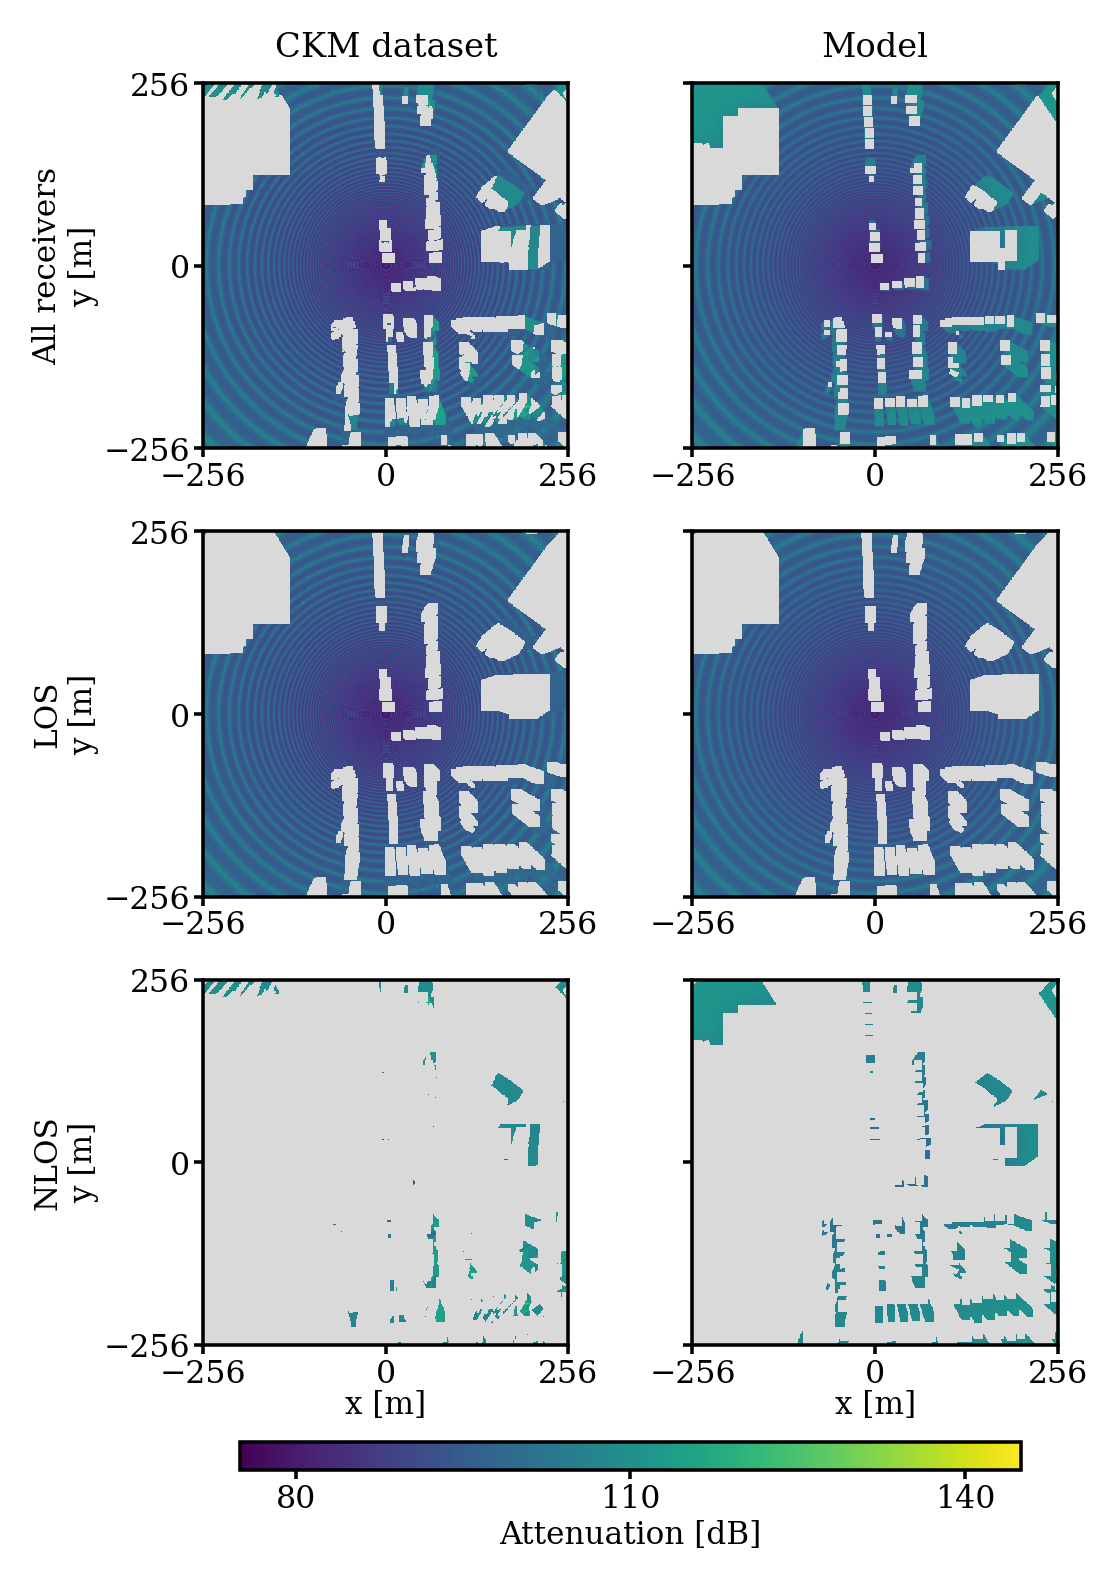
\includegraphics[width=\columnwidth]{figures/nlos_heldout_example.png}
\caption{Held-out Vancouver \texttt{sample\_15142}
($h_{\mathrm{tx}}=\SI{52.22}{m}$; suburban, low-transmitter regime). The dataset
column shows only stored valid targets, while the model column predicts every
ground receiver. Thus, gray in the first dataset panel denotes buildings or
an unavailable target; in the first model panel it denotes buildings only.
Lower rows additionally exclude the other visibility class. Metrics use valid
targets only. The map has 198083 LOS and 12614 NLOS targets; full, LOS, and
NLOS RMSE are 1.85, 1.60, and \SI{4.11}{dB}.}
\label{fig:output_example}
\end{figure}

\subsection{Experimental Setup and Evaluation Protocol}
The dataset split contains 10,840 maps from 37 training cities, 2,750 maps from
15 validation cities, and 2,590 maps from 14 final test cities. No city is moved
between these partitions to ensure strict spatial generalization. The
calibration procedure described in Section~\ref{sec:ckm_model} uses only
training cities, where all nine topology and height regimes are fitted on the
10,840 CKM training samples. The validation subset is reserved for development
checks and component ablation. Final performance results use exclusively the
unseen 14-city test subset.

After excluding building interiors and outdoor channels lacking valid ray
tracing targets, the test dataset contains $423\,087\,119$ valid ground
receivers: $391\,721\,805$ LOS and $31\,365\,314$ NLOS. Thus, 7.413\% of the
evaluated receivers are NLOS because of the elevated UxNB geometry. Although
the pixel-weighted overall score is therefore LOS-dominated, 424 of the 2,590
test maps contain more than 25\% valid NLOS receivers, motivating separate
regime-specific evaluation. An example of the model output is shown in
Fig.~\ref{fig:output_example}.

\subsection{Ablation Study}
Component ablation on the 2,750-map validation set confirms the necessity of
the calibrated terms. Incorporating the coherent ground-reflection term reduces
LOS RMSE from \SI{3.790}{dB} to \SI{1.741}{dB}. On the final test set, raw
COST~231 yields an NLOS RMSE of \SI{25.0098}{dB}, whereas COST~231 augmented
with the fitted regression coefficients and topology- and height-specific
calibration reaches \SI{3.5363}{dB}.

\subsection{Prediction Accuracy and Height Generalization}
The prediction performance on the unseen test set across the standard ITU UxNB
altitude regimes is summarized in Table~\ref{tab:height}. Overall, the proposed
height-aware simulator achieves a global RMSE of \SI{1.9289}{dB}
(\SI{1.7370}{dB} for LOS and \SI{3.5363}{dB} for NLOS). Per-city overall RMSE
ranges from \SI{1.6149}{dB} in Halifax to \SI{2.5851}{dB} in Osaka, with an
unweighted 14-city mean of \SI{1.9831}{dB}. Across the low, medium, and high
altitude groups, overall RMSE decreases from \SI{2.1437}{dB} to
\SI{1.7117}{dB}.

Furthermore, Table~\ref{tab:itu-topology} breaks down final test error by
standard ITU topology. Suburban layouts exhibit the lowest overall error
(\SI{1.6977}{dB}), while dense urban layouts present the harshest NLOS
environment (\SI{4.1319}{dB}), validating topology-specific regime
calibration. The fitted coefficient vectors also change substantially across
topologies, so one global set of slopes would mix distinct relationships. A
compact model retaining eight of the 14 features preserves over 90\% of the
complete model's improvement over a single global NLOS constant.

\begin{table}[t]
\centering
\caption{RMSE [dB] by standard ITU UxNB altitude regime.}
\label{tab:height}
\scriptsize
\setlength{\tabcolsep}{3.5pt}
\begin{tabular}{lrrrr}
\toprule
UxNB height & Overall & LOS & NLOS & Test maps \\
\midrule
Low ($h_{\mathrm{tx}}\le\SI{60}{m}$) & 2.1437 & 1.7923 & 3.7526 & 899 \\
Medium ($\SI{60}{m}<h_{\mathrm{tx}}\le\SI{100}{m}$) & 1.9682 & 1.7747 & 3.5080 & 773 \\
High ($h_{\mathrm{tx}}>\SI{100}{m}$) & 1.7117 & 1.6697 & 2.7620 & 918 \\
\midrule
All heights & 1.9289 & 1.7370 & 3.5363 & 2590 \\
\bottomrule
\end{tabular}
\end{table}

\begin{table}[t]
\centering
\caption{RMSE [dB] by standard ITU topology.}
\label{tab:itu-topology}
\scriptsize
\setlength{\tabcolsep}{3.5pt}
\begin{tabular}{lrrrr}
\toprule
Topology & Overall & LOS & NLOS & Test maps \\
\midrule
Suburban & 1.6977 & 1.6048 & 3.1632 & 1455 \\
Urban & 2.2963 & 1.9967 & 3.6466 & 940 \\
Dense urban & 2.5716 & 2.1126 & 4.1319 & 195 \\
\midrule
All topologies & 1.9289 & 1.7370 & 3.5363 & 2590 \\
\bottomrule
\end{tabular}
\end{table}

\begin{table}[t]
\centering
\caption{Reported RMSE [dB]. Only the first two rows share a test contract.}
\label{tab:accuracy-context}
\scriptsize
\setlength{\tabcolsep}{1.5pt}
\begin{tabular}{@{}>{\raggedright\arraybackslash}p{1.55cm}>{\raggedright\arraybackslash}p{1.95cm}rrr@{}}
\toprule
Method & Evaluation contract & All & LOS & NLOS \\
\midrule
Proposed & CKM city holdout & 1.9289 & 1.7370 & 3.5363 \\
GMM U-Net & Same split and masks & 4.3606 & 4.4323 & 3.3381 \\
RadioUNet & RadioMapSeer DPM & 1.60 & -- & -- \\
RadioVAE$_C$ & RadioMapSeer DPM & 1.42 & -- & -- \\
TSRDiff & BRAT-Lab, 10\% samples & 3.62 & -- & -- \\
RO-HMTGP & Measured RSRP & 4.19--6.00 & -- & -- \\
\bottomrule
\end{tabular}
\end{table}

The GMM U-Net is a controlled neural alternative: a height-conditioned mixture
head and U-Net decoder, separated into six topology classes and LOS/NLOS
experts, are evaluated on the same 2590 maps and masks. It was the best purely
neural approach in an internal exploration of over 50 configurations. Its
lower NLOS error shows where distribution-aware learning can help, while the
lower LOS and overall errors of the proposed model show the value of resolving
the stable coherent component explicitly. A following paper will study a
hybrid model using calibrated attenuation, delay spread, and angular spread
priors as inputs and base estimates for neural refinement.

The remaining rows are published context, not a controlled ranking. RadioUNet
and RadioVAE~\cite{radiounet2020,radiovae2025} use $256^2$ fixed-height
terrestrial RadioMapSeer data; TSRDiff~\cite{tsrdiff2025} uses sparse targets,
and RO-HMTGP~\cite{rohmtgp2025} predicts measured RSRP rather than dense
simulated attenuation. Their values indicate scale under different tasks, not
superiority over the present $513^2$ variable-height city holdout.

\subsection{Computational Complexity}
Table~\ref{tab:compute} compares the proposed simulator with MATLAB ray tracing
and deep learning baselines. CPU timings use the same AMD Ryzen 5 5600X with GPU
disabled; neural timings exclude file I/O and use 10 warmups and 50 forward
passes. The proposed model executes in \SI{0.0602}{s} per $513^2$ map.

\begin{table}[!t]
\centering
\caption{Computational context; reported CPU rows use the same CPU.}
\label{tab:compute}
\scriptsize
\setlength{\tabcolsep}{2.2pt}
\begin{tabular}{@{}lcrrr@{}}
\toprule
Method & Grid & State & Reported MAC & CPU [s] \\
\midrule
Proposed & $513^2$ & 66.8k+126 & 0.170M$^\ast$ & 0.0602 \\
RadioUNet~\cite{radiounet2020} & $256^2$ & 13.27M & 12.73G & 0.1339 \\
PMNet~\cite{pmnet2023} & $256^2$ & 33.34M & 52.71G & 0.4042 \\
SSL-Radio~\cite{sslradio2025} & $256^2$ & 15.4--20.4M & 16.9--21.9G$^\dagger$ & -- \\
MATLAB RT & $513^2$ & -- & -- & 102.289 \\
\bottomrule
\end{tabular}
\end{table}
The proposed state is 66800 LOS lookup values plus 126 NLOS coefficients. The
asterisk counts the final NLOS dot products, while the measured time includes
feature construction and LOS evaluation; the dagger is reconstructed from the
published layer table. MATLAB RT also generates visibility and three channel
quantities, so its raw $\sim1700\times$ gap is significant but not a like-for-like
attenuation speedup.

\subsection{Scope and Limitations}
The reported accuracy is conditional on the supplied RT visibility mask. For
fixed city geometry, transmitter position and height, receiver grid, and RT
settings, that mask is deterministic and can be stored once; all 742392 values
matched in a five-condition audit. The fitted tables inherit the simulator,
antenna, carrier, terrain, and building products, while COST231 is only a
calibrated basis outside its original domain. The result is therefore a
transparent dataset baseline and refinement anchor, not a universal propagation
law.

\section{Conclusions}\label{sec:conclusions}
This paper introduced a dense FR3 (\SI{7.125}{GHz}) UAV CKM dataset providing
attenuation, delay spread, angular spread, geometric visibility, building
geometry, transmitter height, and topology labels across 16,180 simulated
samples from 66 global cities. Using this dataset, we proposed a computationally
efficient, height-aware attenuation prediction framework. By relying on
conventional propagation models calibrated on the dataset, the model generates
accurate attenuation maps and generalizes to unseen city layouts. It achieves
an overall test RMSE of \SI{1.9289}{dB} and executes in \SI{0.0602}{s} per map
on a CPU. The results further show that topology is the principal NLOS
calibration partition, with transmitter height refining that partition and the
regional morphology scale carrying most of the useful local context.

The model is intended as a physical/statistical base rather than a rejection of
deep learning. The controlled GMM U-Net result identifies NLOS as the promising
refinement target, but also shows the cost of asking a network to relearn the
coherent LOS field. A future journal paper will train distribution-aware
networks to refine analogous calibrated priors for attenuation, delay spread,
and angular spread. Its multi-output runtime will not be directly comparable to
this attenuation-only benchmark, but the present computational gap shows that
the prior-first strategy is significant and worth preserving.

\bibliographystyle{IEEEtran}
\bibliography{references}

\end{document}
